\documentclass[11pt,dvipdfmx]{jreport}
\usepackage{wuse_thesis}
\usepackage{indentfirst}
\usepackage{url}	% \url{}コマンド用.URLを表示する際に便利
\usepackage{graphicx}  % ←graphicx.styを用いてEPSを取り込む場合有効にする
\usepackage{color}
\usepackage{listings}
\usepackage{multirow}
% \usepackage{caption} 

\renewcommand\lstlistingname{Program}
\newcommand{\todo}[1]{\colorbox{yellow}{{\bf TODO}:}{\color{red} {\textbf{[#1]}}}}

			% 他のパッケージ・スタイルを使う場合には適宜追加

%%%%%%%%%%%%%%%%%%%%%%%%%%%%%%%%%%%%%%%%%%%%%%%%%%%%%%%%%%%%%%%%%%%%%%%%

%%
%% 主に表紙を作成するための情報
%%

%%  タイトル(修論の場合は英語表記も指定)
\title{複数プロジェクト開発履歴を用いた\\コーディング規約違反の修正予測精度の評価}
%\etitle{Test\\Test\\Test}

%%  著者名(修論の場合は英語表記も指定)
\author{亀岡 令}
%\eauthor{Akinori Ihara}

%% 卒業論文・修士論文(以下のどちらかを選択)
\bachelar	% 卒業論文(4年生用)

%%  学科・クラスタ
\department{システム工}
%\department{デザイン情報}
%\department{デザイン科学}

%%  学生番号
\studentid{60256065}

%%  卒業年度
\gyear{2023}		% 提出年が2022年なら,2021年度

%%  論文提出日
\date{2024年2月13日}	% 修士の場合は月(2021年2月)までとし,英語表記も指定
%\edate{February 2021}	% 修士の場合,こちら(英語表記)も有効化

%%%%%%%%%%%%%%%%%%%%%%%%%%%%%%%%%%%%%%%%%%%%%%%%%%%%%%%%%%%%%%%%%%%%%%%%

\begin{document}

\maketitle

%%
%%  概要
%%
\begin{abstract}

\todo{はじめにと一緒に最後に書く}
複数の開発者が参画するソフトウェア開発では.開発者は可読性,保守性の向上のために静的解析ツールを用いてコーディング規約に違反しているソースコードを検出し,修正に取り組む.しかし,静的解析ツールは規約違反の指摘漏れを抑えるため,大量の規約違反を出力し,その大半が開発者に修正されていない.従来研究では,規約違反を検証するプロジェクトの過去の修正履歴を学習したモデルを構築し,静的解析ツールの検出結果の中で優先的に修正すべき規約違反ソースコードを予測する手法を提案している.本研究では,従来研究において単一プロジェクトの学習によって十分に学習できない規約違反を,複数プロジェクトのデータの学習する予測モデルを構築し,当該モデルが多様な規約違反を予測可能か否かを明らかにする.
\todo{結果関係}

\end{abstract}

%%  目次
\tableofcontents

%%  図目次 (図目次をいれたければ以下のコメントをはずす)
%\listoffigures

%%  表目次 (表目次をいれたければ以下のコメントをはずす)
%\listoftables

\newpage
\pagenumbering{arabic}	% 以降のページ番号を算用数字に


%%%%%%%%%%%%%%%%%%%%%%%%%%%%%%%%%%%%%%%%%%%%%%%%%%%%%%%%%%%%%%%%%%%%%%%%

%%
%%  本文はここから
%%

\chapter{はじめに}

コーディング規約とは,ソースコードを一定の品質に保つための記述方法について,禁止事項や推奨事項,保守性を高めるためのコーディングスタイルなどを定めたものである.
コーディング規約は各プログラミング言語ごとに存在し,代表的なコーディング規約が複数存在することもある.例えば,Java言語のJavaコーディング標準,Python言語のPEP8などがある.これらコーディング規約には命名規則やコメント文などに関するルールが定められている.
オープンソースソフトウェアやチームでのソフトウェア開発において,開発者はコーディングスタイルの共通化や,プログラムの最適化のためにコーディング規約に従いながらコーディングすることが多い.コーディング規約を遵守することによって,ソースコードの可読性が向上し,ソフトウェア保守が容易になることが知られている\cite{EffectsSAT}.

従来研究では,プロジェクトへのコーディング規約の導入によって,ソフトウェア開発におけるソースコードの理解の促進,バグの早期発見などに効果があることを明らかにしている\cite{Beller2}\cite{Johnson}\cite{Beller}.

開発現場においてソースコードがコーディング規約に違反している箇所を検出するためには静的解析ツールが用いられる.
静的解析ツールはソースコードを実行することなく,ソースコードに含まれるコーディング規約に違反している箇所を検出することができ,継続的インテグレーションのプロセスの1つとして使用されることも多い.
開発者は自動的に検出された違反を確認することで,コーディング規約違反箇所を速やかに修正することができる.

静的解析ツールは,ソースコードからすべてのコーディング規約に違反しているコード断片を検出する.
静的解析ツールは多くの規約の種類を定義しているため,誤検出を含む大量の規約違反検出結果が出力されることが頻繁に発生する.
そのため,開発者はその多くを修正せずに放置している.
静的解析ツールの誤検出は開発効率の低下につながるため,検出精度を向上させるための研究が行われている\cite{Nguyen}.

従来研究では大量に検出されるコーディング規約違反の中から,機械学習を用いて優先して修正すべき違反かそうでない違反の2値に分類する手法を提案している\cite{JyuraiPre}.他にも静的解析ツールの検出結果を優先度づけする研究は数多く行われている.
従来研究の多くは,単一プロジェクトの開発履歴を学習することで各プロジェクトのコーディングの慣習を捉えた予測を行っているが,単一プロジェクトの開発履歴のみを習データとしているため,十分なデータが集まらなかった場合に学習不足に陥ることが考えられる.
そこで,Tabassumらは,不具合予測やプログラムの自動修正において,データ不足,コールドスタート問題への対応として,異なるプロジェクトの開発データを用いることによって学習データを補う手法を提案している\cite{Tabassum}.
ただし,複数プロジェクトのデータを用いることによって,実装方針の異なるプロジェクトのデータを学習することとなるため,十分なデータがある場合には,単一プロジェクトのデータのみを学習したほうが高い予測精度を得ることができる.

本研究では,複数プロジェクトの開発データを予測モデルの学習に使用することによる,コーディング規約違反の修正予測制度への影響を明らかにする.提案手法として2種類の予測モデルを構築する.1つは,複数プロジェクトのデータを単純に結合し,学習するモデル構築手法である.もう1つは,複数プロジェクトのデータを結合後にクラスタリングを行い,各クラスタごとに予測モデルを構築する手法である.各手法の詳細やクラスタリングを行う理由については\ref{chap:approach}章にて説明する.

つづく\ref{chap:background}章では,本研究の位置付け,および従来研究を述べる.\ref{chap:approach}章では,提案手法の詳細な学習データの作成方法や機械学習モデルの作成方法の説明を行う.\ref{chap:result}章では,従来手法である単一プロジェクトのデータのみを学習する手法と提案手法である複数プロジェクトのデータを学習する手法を用いた修正予測を行い,手法ごとのモデルの精度および予測内容の分析を行った結果を示す.\ref{chap:consideration}章では,結果に基づく考察を行い,\ref{chap:heuristic}章では本研究の妥当性への脅威について述べ,\ref{chap:end}章でまとめる.

%-----------------------------------prev
% 複数人で実装するソフトウェア開発では,開発者間のコーディングスタイルを共通化することにより,ソースコードの可読性を高め,ソフトウェア保守が容易になることが知られている\cite{EffectsSAT}.コーディングスタイルを共通化するため,各プログラミング言語ではソースコードを記述するためのガイドラインとしてコーディング規約を公開している.具体的には,Java言語のJavaコーディング標準,Python言語のPEP8などがある.これらコーディング規約には命名規則やコメント文などに関するルールが定められている.

% 従来研究では,コーディング規約の導入により,ソフトウェア開発プロジェクトにとってソースコード理解の促進,バグの早期発見などに効果があることを明らかにしている\cite{Beller2}\cite{Johnson}\cite{Beller}.

% コーディング規約に従って実装しているか否かの判定には,多くのプロジェクトで静的解析ツールが用いられている.静的解析ツールは,ソースコードを実行することなく,ソースコード中に含まれるコーディング規約の違反箇所やバグを検出することができ,継続的インテグレーションのプロセスの一つとして使用されることも多い.開発者は,静的解析ツールが検出した規約違反を修正することでプロジェクトの実装方針に従った共通のコーディングスタイルで実装することができる.しかし,多くのプロジェクトでは,規約違反の指摘漏れを抑えるために規約違反の判定基準を厳しく設定しており,静的解析ツールは大量の規約違反を出力し,開発者はその多くを修正していないことが課題として挙げられる.このような静的解析ツールの誤検出を防ぐための研究が数多く発表されている\cite{Nguyen}.

% 従来研究では,機械学習や深層学習を用いて,大量に検出されたコーディング規約違反の中から優先して修正すべき違反とそれ以外の違反の2クラス分類する手法を提案している.このように静的解析ツールの検出結果を優先順位づけする研究は多数行われているが,予測精度が低いことが課題である.この課題の原因の一つとして,従来研究では機械学習モデルの構築において,予測するプロジェクトと同じプロジェクトを学習データに用いるため,データセットサイズや修正される違反の割合が少ない場合に十分な学習ができずに予測精度が下がってしまうことが考えられる.

% 単一プロジェクトでは,一部の規約違反の発生および修正が少ないため十分な学習データを確保できない.そこで,不具合予測やプログラム自動修正などの研究では,データ不足,コールドスタート問題への対応として,異なるプロジェクトの開発履歴を用いることで学習データを補う手法が提案されている\cite{Tabassum}.

% ただし,同一プロジェクトのデータは,プロジェクトの実装方針が同一のため,異なるプロジェクトの開発履歴を用いるよりも高い精度が得られる.

% 本研究では,複数プロジェクトの開発履歴を用いて,修正を要する規約違反ソースコードを特定する手法を提案し,評価する.具体的には複数プロジェクトにおける規約違反の修正履歴を統合したモデル,および各規約違反したソースコードの特徴に基づきクラスタリングすることによって規約違反を修正する特徴が類似するモデルを構築し,それぞれの手法による予測精度を分析する.ケーススタディとして,Python言語で記述されたオープンソースソフトウェア10プロジェクトを対象に予測モデルを構築し予測性能を評価した.

% つづく\ref{chap:background}章では,本研究の位置付け,および従来研究を述べる.\ref{chap:approach}章では,提案手法の詳細な学習データの作成方法や機械学習モデルの作成方法の説明を行う.\ref{chap:result}章では,従来手法と提案手法および提案手法を用いずにすべての学習データを結合したものをそれぞれ学習データとした修正優先度予測を行い,手法ごとのモデルの精度および予測内容の分析を行った結果を示す.\ref{chap:consideration}章では,結果に基づく考察を行い,\ref{chap:heuristic}章では本研究の妥当性への脅威について述べ,\ref{chap:end}章でまとめる.
%-----------------------------------


\chapter{コーディング規約と静的解析ツール}\label{chap:background}
\section{コーディング規約違反}


\begin{figure}[t]
% \small
\vspace{-16pt}
    \begin{lstlisting}[caption={[upper/lower text]%
               \begin{tabular}[t]{@{}l@{}}
                problematic.py \\[1.0\normalbaselineskip]
               \end{tabular}},frame={tb},numbers=left,label=problematic,identifierstyle={\small}]
def print_fruits():
    fruit1 = "orange"
    fruit2 = "apple" # [unused-variable]
    print(fruit1)
\end{lstlisting}
\vspace{-8mm}
\end{figure}

\begin{figure}[t]
% \small
    \begin{lstlisting}[caption={[upper/lower text]%
               \begin{tabular}[t]{@{}l@{}}
                correct.py \\[1.0\normalbaselineskip]
               \end{tabular}},frame={tb},numbers=left,label=correct,identifierstyle={\small}]
def print_fruits():
    fruit1 = "orange"
    fruit2 = "apple"
    print(fruit1, fruit2)
\end{lstlisting}
% \vspace{-4mm}
\end{figure}



コーディング規約とは,企業や開発チームのような複数人でプロジェクト開発を行う際に,プログラミングにおける規則についてまとめたものである.
規約の中には変数やクラス,関数などの命名規則について定めたものや,その他に禁止事項,制限事項,推奨事項などが定義されている.
コーディング規約には,コードの構造やコーディングスタイルなどを共通化させるためのルールが定められており,プログラミング言語ごとに複数存在している.例えばPython言語のPEP8,Java言語のCode Conventions for the Java Programming LanguageやGoogle Java Style Guide,JavaScript言語のGoogle JavaScript Style GuideやAirbnb JavaScript Style Guideのようにプログラミング言語ごとに違反の`種類'や`基準'が異なる規約が複数存在する.開発者は複数存在するコーディング規約から自身のプロジェクトやコーディングスタイルに適したコーディング規約を選んで利用している.

次にコーディング規約への違反の例とその修正例を示す.Program \ref{problematic},\ref{correct}はPythonのコーディング規約PEP8に違反しているコードと修正した例である.
また,静的解析ツールのPylintの公式文書であるPylint 2.17.5 documentation\footnote{https://pylint.readthedocs.io/en/stable/index.html}に掲載されているコーディング規約への違反・修正例である.
ここで掲載している違反はプログラム中に利用されていない変数が宣言されている場合に検出される違反である.
Program \ref{problematic}で宣言されている変数\texttt{`fruit2'}は利用されておらず,利用するように修正したコードがProgram \ref{correct}である.この例では\texttt{`fruit2'}を削除することでも解消される.

コーディング規約違反の検出は開発者が目視で行うには多くのコストを要するため,静的解析ツールが用いられる.静的解析ツールはソフトウェアのコードを実行することなくコード中に含まれるエラーや脆弱性を含むコードを検出することができる.静的解析ツールにも各言語ごとに複数の種類があり,参照している規約の種類や,違反を検出した際のメッセージのフォーマットや,検出する違反のカスタマイズ性の高さなどが異なる.

%-----------------------------------prev
% コーディング規約は,ソフトウェア開発プロジェクトがソースコードの可読性や保守性の向上を目的に,コーディングスタイルを共通化するためのルールとして使用される.規約には,ソースコードの構造から命名規則などのコーディングスタイルについて,禁止事項,制限事項,推奨事項などがルールとして含まれる.各プログラム言語がそれぞれ推奨するコーディング規約を公開している.Java言語はJavaコーディング標準,Google Java Style Guide,C言語はMISRA-C,CERTコーディングスタンダード,C++言語はMISRA-C++,Python言語はPEP8などを提供している.共同開発するプロジェクトは,それぞれの方針に合わせてプログラム言語別に推奨されるコーディング規約を適宜拡張して使用している.

% コーディング規約には検出漏れを防ぐために多数のルールがあり,開発者がコーディング規約を違反しているソースコードを目視で発見することは困難である.そのため,コーディング規約に従って実装されているか否かの判定には多くのプロジェクトで静的解析ツールの使用が推奨されている\cite{Beller}.
% 静的解析ツールは,ソースコードを実行することなく,規約違反しているソースコードを網羅的に検出することができる.コーディング規約と同様,各プログラミング言語には,それぞれ規約に違反するソースコードを検出する静的解析ツールが存在する.Java言語はCheckStyle,PMD,FindBugs,C言語はQAC,CX-Checker,Python言語はflake8,JavaScript言語はESLintなどがある.静的解析ツールは低コストで導入できるため,多くの組織で導入されている\cite{UsingStaticAnalysisTools1}\cite{UsingStaticAnalysisTools2}.
%-----------------------------------

\section{静的解析ツールの問題点}

開発環境において静的解析ツールを用いて開発するには問題点が存在する.静的解析ツールは各違反ごとに書かれたルールに合致した場合にすべて違反として検出し出力するため,大量の検出結果が出力されることが頻繁に発生する.実際に多くのプロジェクトで静的解析ツールのルールを変更することなく利用するため,静的解析ツールが大量の規約違反を検出することが多い\cite{UsingStaticAnalysisTools2}.
大量の違反の検出結果には誤検出も含まれ,それらを開発者がレビューし修正するには多くのコストを要するため困難である.さらに様々な違反から優先して修正すべき規約違反を特定することは,開発の経験や,プロジェクトごとに異なるコーディングスタイルの理解などが必要であるため,共同開発者にとっても容易でない\cite{shuseisarenai}.

従来研究では各プロジェクトごとに異なる優先して修正すべき規約違反の特定のために,機械学習モデルを用いた特定手法などが数多く提案されている.

%-----------------------------------prev
% 静的解析ツールは効率的に規約違反を検出できる一方で,多くのプロジェクトは静的解析ツールが定義する膨大な規約違反の検出ルールを変更することなく利用しているため,静的解析ツールが多量の規約違反を検出することが多い\cite{UsingStaticAnalysisTools2}.
% その結果,検出された規約違反の多くは開発者によって修正されないままとなり,修正されないままの規約違反は静的解析ツールの誤検出として取り扱われる.このように膨大な規約違反の中から優先的に修正する規約違反を特定するためには,開発者の実装経験,プロジェクトの慣習の理解が必要であり,共同開発する開発者にとって容易な作業ではない\cite{shuseisarenai}.優先的に修正される規約違反の特定に向けて,多くの従来研究が機械学習モデルなどを用いた特定手法を提案している.
%-----------------------------------


\section{従来手法}

静的解析ツールの誤検出を含む大量の検出結果によって開発効率の低下を防ぐため,Ruthruffらは機械学習モデルを用いて優先して修正すべき違反を特定する手法を提案している\cite{JyuraiPre}.
その他,Kimらは静的解析ツールの出力結果をベイジアンネットワークに活用することにより,規約違反しているコードの修正優先度の予測を行う手法が提案されている\cite{beizu}.
これらの研究のほかにも静的解析ツールによって検出された規約違反コードの修正優先度付けを行う研究や,修正の要否を予測する研究は数多く行われている\cite{Wang}\cite{Qing}\cite{HowFar}.
機械学習のモデル構築には,規約違反コードの優先度予測対象のプロジェクトの過去の開発履歴を学習データとし,新しいデータを評価用データとすることで構築したモデルの評価を行っている.
本研究では,Ruthruffらの従来手法と同様に,説明変数としてソースコードの特徴量などを利用し,規約違反コードの修正の必要の要否を予測する2クラス分類モデルを構築し,評価を行う.

従来手法では,予測対象とするプロジェクトの過去の開発履歴を学習データとして,予測モデルを構築している.各プロジェクトにはコーディングスタイルなどが存在し,修正の要否はプロジェクトことに異なることが考えられるため,評価用データと同じプロジェクトのデータを学習するほうが,他プロジェクトのデータを学習するより高い予測精度が得られると考えられる.
しかし,評価用データと同じプロジェクトを学習データとする場合,出現する規約違反の種類や,各違反の修正率が大きく異なる\cite{Panichella}.そのため,規約違反が修正される(正例)と修正されない(負例)の数が不均衡になる場合や,データサイズが小さいことにより,十分な学習ができず予測性のが低下することが示唆される.

本研究では,予測モデルの構築の際に用いる学習データに評価用データとは異なる別プロジェクトの開発履歴を用いることにより,規約違反コードの修正用品も予測を行う.名倉らは,複数プロジェクトを用いてコーディング規約違反の発生の増減の予測を行っているが,発生した違反が修正されるか否かを予測することは行っていないため,予測の点において本研究との差分となっている\cite{nagura}.
複数プロジェクトのデータを学習に用いることで学習データの拡張を図ることができ,予測精度の向上を見込むことができるが,プロジェクトごとの各違反に対する修正優先度は異なるため,複数プロジェクトのデータを用いることによって予測精度が低下することも考えられる.そこで,本研究では複数プロジェクトの開発データを学習した場合の予測精度への影響を明らかにすることを目的とする.

%-----------------------------------prev
% 静的解析ツールの誤検出による開発効率の低下を防ぐため,Ruthruffらは機械学習モデルを用いて優先的に修正される規約違反を含むコード断片の特定手法を提案している\cite{JyuraiPre}.その他,Kimらはベイジアンネットワークと静的解析ツールを用いて規約違反コード断片の修正優先度を予測する手法を提案している\cite{beizu}.これらのように静的解析ツールによって検出された結果に対して優先順位付けを行う研究は数多く行われている\cite{Wang}\cite{Qing}\cite{HowFar}.機械学習モデルの構築では,特定のプロジェクトの分析対象期間中に検出された規約違反の修正履歴を用いて機械学習モデルを構築している.分析対象期間中の古い時期の記録を学習データ,新しい時期の記録を評価データとしてモデルを構築,評価している.本研究では,Ruthruffらの従来研究と同様に,ソースコードの特徴量などを説明変数として使用し,規約違反コード断片の修正優先度が高いか否かを予測する2クラス分類モデルを構築する.

% 従来手法では,評価対象とするプロジェクトにおける過去の開発履歴を学習データとして,修正を要する規約違反を予測するモデルを構築している.機械学習モデルを取り扱う上で,評価データと同一のプロジェクトの開発履歴を使用するほうが,異なるプロジェクトの開発履歴を用いるよりも高い精度が得られることが知られている.しかし,過去の開発履歴を学習データとして使用する場合,規約の種類によって規約違反の修正率,修正数が大きく異なる\cite{Panichella},その結果,規約違反が修正されるコード断片(正例),規約違反が修正されないコード断片(負例)の数が不均衡となり,機械学習モデルの予測性能が低下することが示唆される.

% 本研究では,学習データに評価対象とは異なるプロジェクトの開発履歴も使用することにより,修正を要するか否かを判別するモデルを構築する.名倉らは,複数プロジェクトを用いてコーディング規約違反の増減を予測しているが,その違反が修正されるかは予測していないため,その点が本研究との差分となる\cite{nagura}.学習データを増やすことで修正する規約違反のコード断片の特定精度の向上が期待できる.その一方で,プロジェクトに応じて実装や違反に対する修正の慣習が異なるため,異なるプロジェクトの開発履歴が予測精度の低下を招くことも考えられる.本研究では複数プロジェクトのデータを学習した際の予測精度への影響を明らかにするために本研究において検証する.
%-----------------------------------



\chapter{修正を要する規約違反ソースコードの特定手法}\label{chap:approach}

\section{概要}

\begin{figure*}[t]
	\centering
	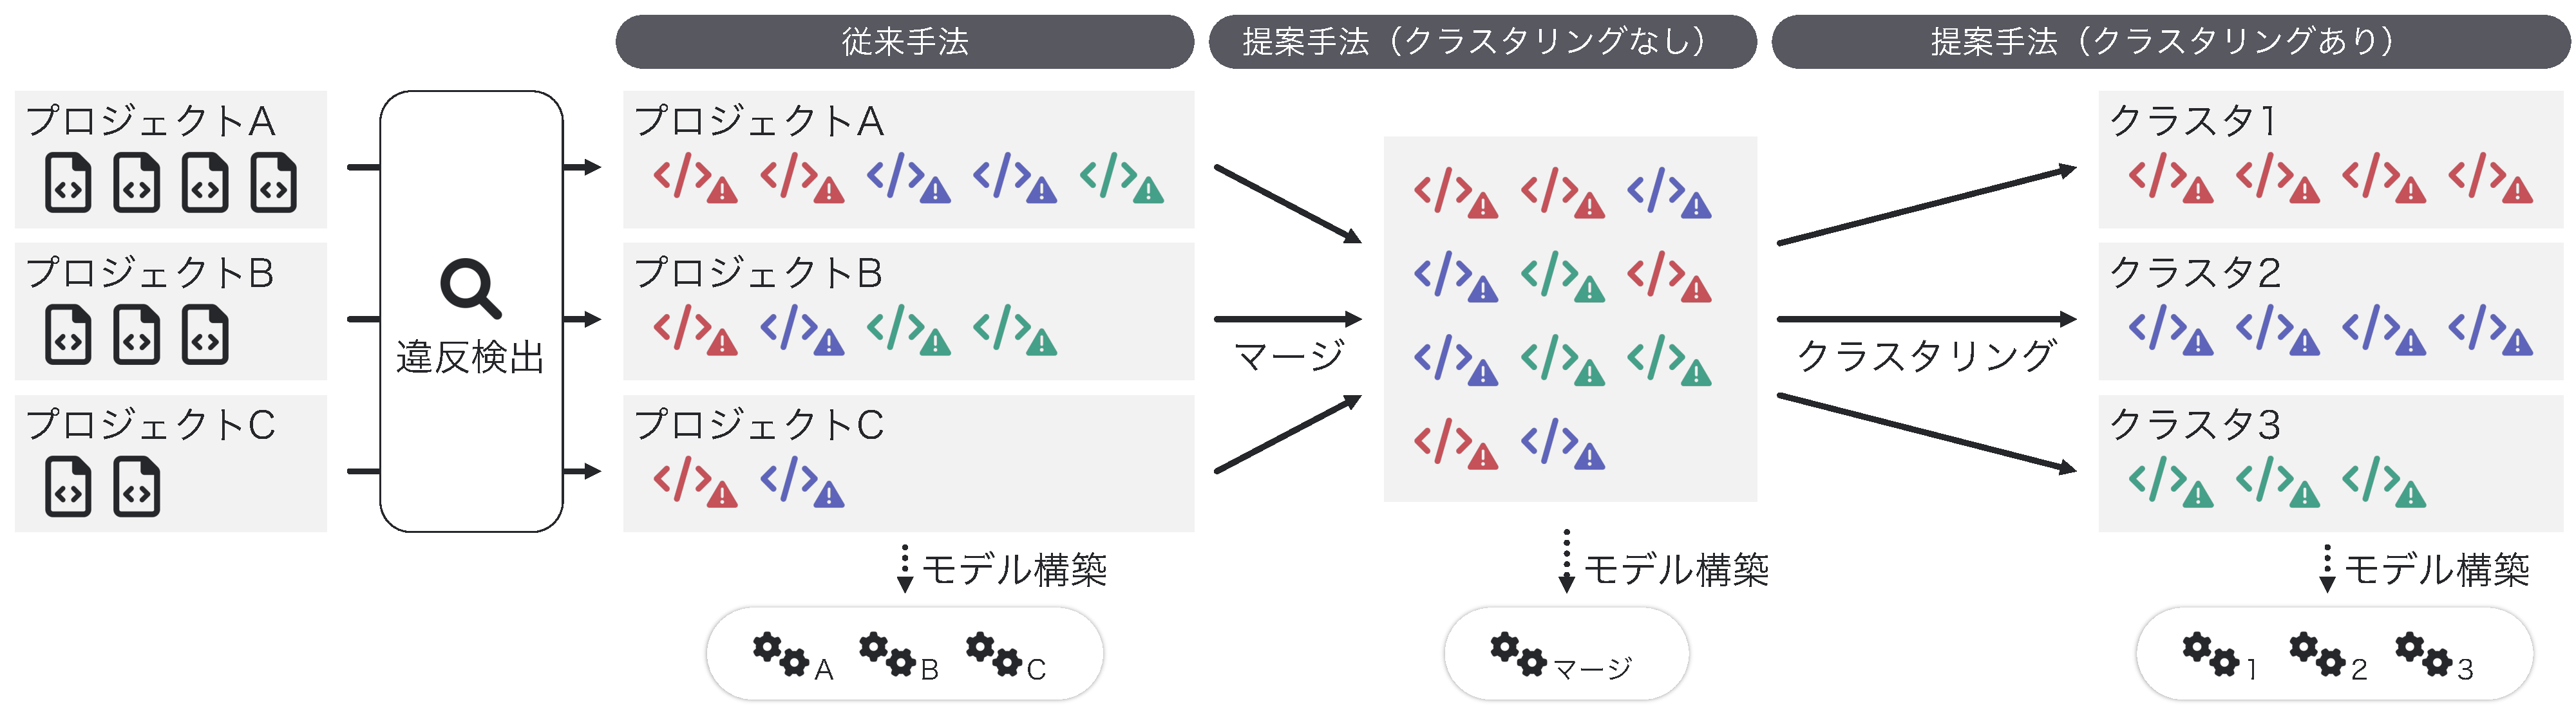
\includegraphics[width=1.0\linewidth]{Kameoka_fig/kameoka_fig1.pdf}
	\caption{本研究の概略図}
	\label{fig:Teiannsyuhou}
\end{figure*}

本研究の検証手法は図\ref{fig:Teiannsyuhou}の通りである.本研究では,静的解析ツールによって検出されたコーディング規約違反を修正すべき違反かそうでない違反かの2値に分類する機械学習モデルを3種類作成する.各モデルの概要は以下の通りである.

\begin{enumerate}
  \item 従来研究の手法を採用したモデルであり,予測対象のプロジェクトの過去の開発履歴のみを学習することによる予測モデルを構築
  \item 提案手法の複数プロジェクトの開発履歴を学習させる手法で,すべての学習データを結合し学習した予測モデルを構築
  \item 提案手法で複数プロジェクトのデータを結合した後に,クラスタリングを行い各クラスタごとに予測モデルを構築
\end{enumerate}

従来手法1種類と提案手法2種類の予測モデルを作成し,修正の要否を予測し評価する.評価の結果を基に,静的解析ツールの違反検出結果から修正が必要な違反を推薦する予測に対する本研究の有効性を検証する.

提案手法において,複数プロジェクトのデータを学習させる理由は,従来研究では,予測対象のプロジェクトと同プロジェクトの過去のデータを学習しているが,開発履歴がない場合や,違反回数が少ない場合に学習不足,または学習不可になることが発生する.この問題を解決するために,予測対象のプロジェクト以外のデータを学習させることによって学習データを補完する.

次に結合したデータをクラスタリングする理由については,提案手法(クラスタリングなし)では,学習データに複数プロジェクトのデータを用いることによって学習データを拡張しているが,各プロジェクトごとに存在するコーディングスタイルなどの特徴を無視したまま結合している.この問題に対してクラスタリングを用いることによって,説明変数の類似したものを収集することができるため,一定の類似性のあるものから学習することが可能になる.クラスタリングによって作成される説明変数の類似によるクラスタが,各プロジェクトのコーディングスタイルの類似とは言えないが,説明変数同士の類似性を見ることによって,単純に結合した場合より効果的に複数プロジェクトのデータを学習できると考えられるため,提案手法の二段階目としてクラスタリングを用いた手法を採用した.

%-----------------------------------prev
% 図\ref{fig:Teiannsyuhou}は,本研究の提案手法の概略図を示す.本研究では,規約に違反している箇所を修正するか否かを予測する3つの機械学習モデルを構築する.まず,図の左から,各プロジェクトのソースコードを対象に静的解析を行い,規約違反を含むソースコードの特徴量の計測,および,規約違反の修正有無を計測する.次に,学習データとして各プロジェクトの開発履歴のみを用いて機械学習モデル(従来手法)を構築する.続いて,各プロジェクトの開発履歴をすべて統合した学習データを用いた機械学習モデル(提案手法(クラスタリングなし))を構築する.最後に統合した学習データを階層的クラスタリングによって10クラスタに分割し,それぞれのクラスタの開発履歴を用いて機械学習モデル(提案手法(クラスタリングあり))を構築する.本研究では,評価に用いるオープンソースソフトウェアの対象プロジェクト数に合わせてクラスタ数を10としている.また,提案手法のクラスタリングは,全てのプロジェクトの学習データと評価用データを合わせてクラスタリングを行い,評価用データは,分類されたクラスタの学習データで構築したモデルを用いて予測する.
%-----------------------------------

\section{学習データと評価データの収集}

本研究では,複数プロジェクトのデータを学習するにあたって,すべてのプロジェクトのデータを学習に用いるために,各プロジェクトのデータを時系列順に並べた際の古いものから8割を学習に用い,残りの2割を検証用データとして用いた.ここで時系列順に並べている理由は,学習時に本来得られない未来のデータを学習させないために時系列の古いものを学習データとしている.そのため,モデルの評価時に,交差検証は行なっていない.

%-----------------------------------prev
% 本研究では,2種類の提案手法において構築する機械学習モデルにおいて複数のプロジェクトの開発履歴を統合するが,モデル構築に使用する学習データにも,検証に使用する評価データにも全てのプロジェクトが含まれるように考慮する.具体的には,各プロジェクトの分析対象期間に発生するコミットのうち,前半8割を学習データ,後半2割を評価データとし,各プロジェクトにおいて未来のデータを含まないようにするため交差検証を行わない.
%-----------------------------------




\section{説明変数・目的変数の計測方法}


%-------------------------
\begin{figure}[t]
	\centering
	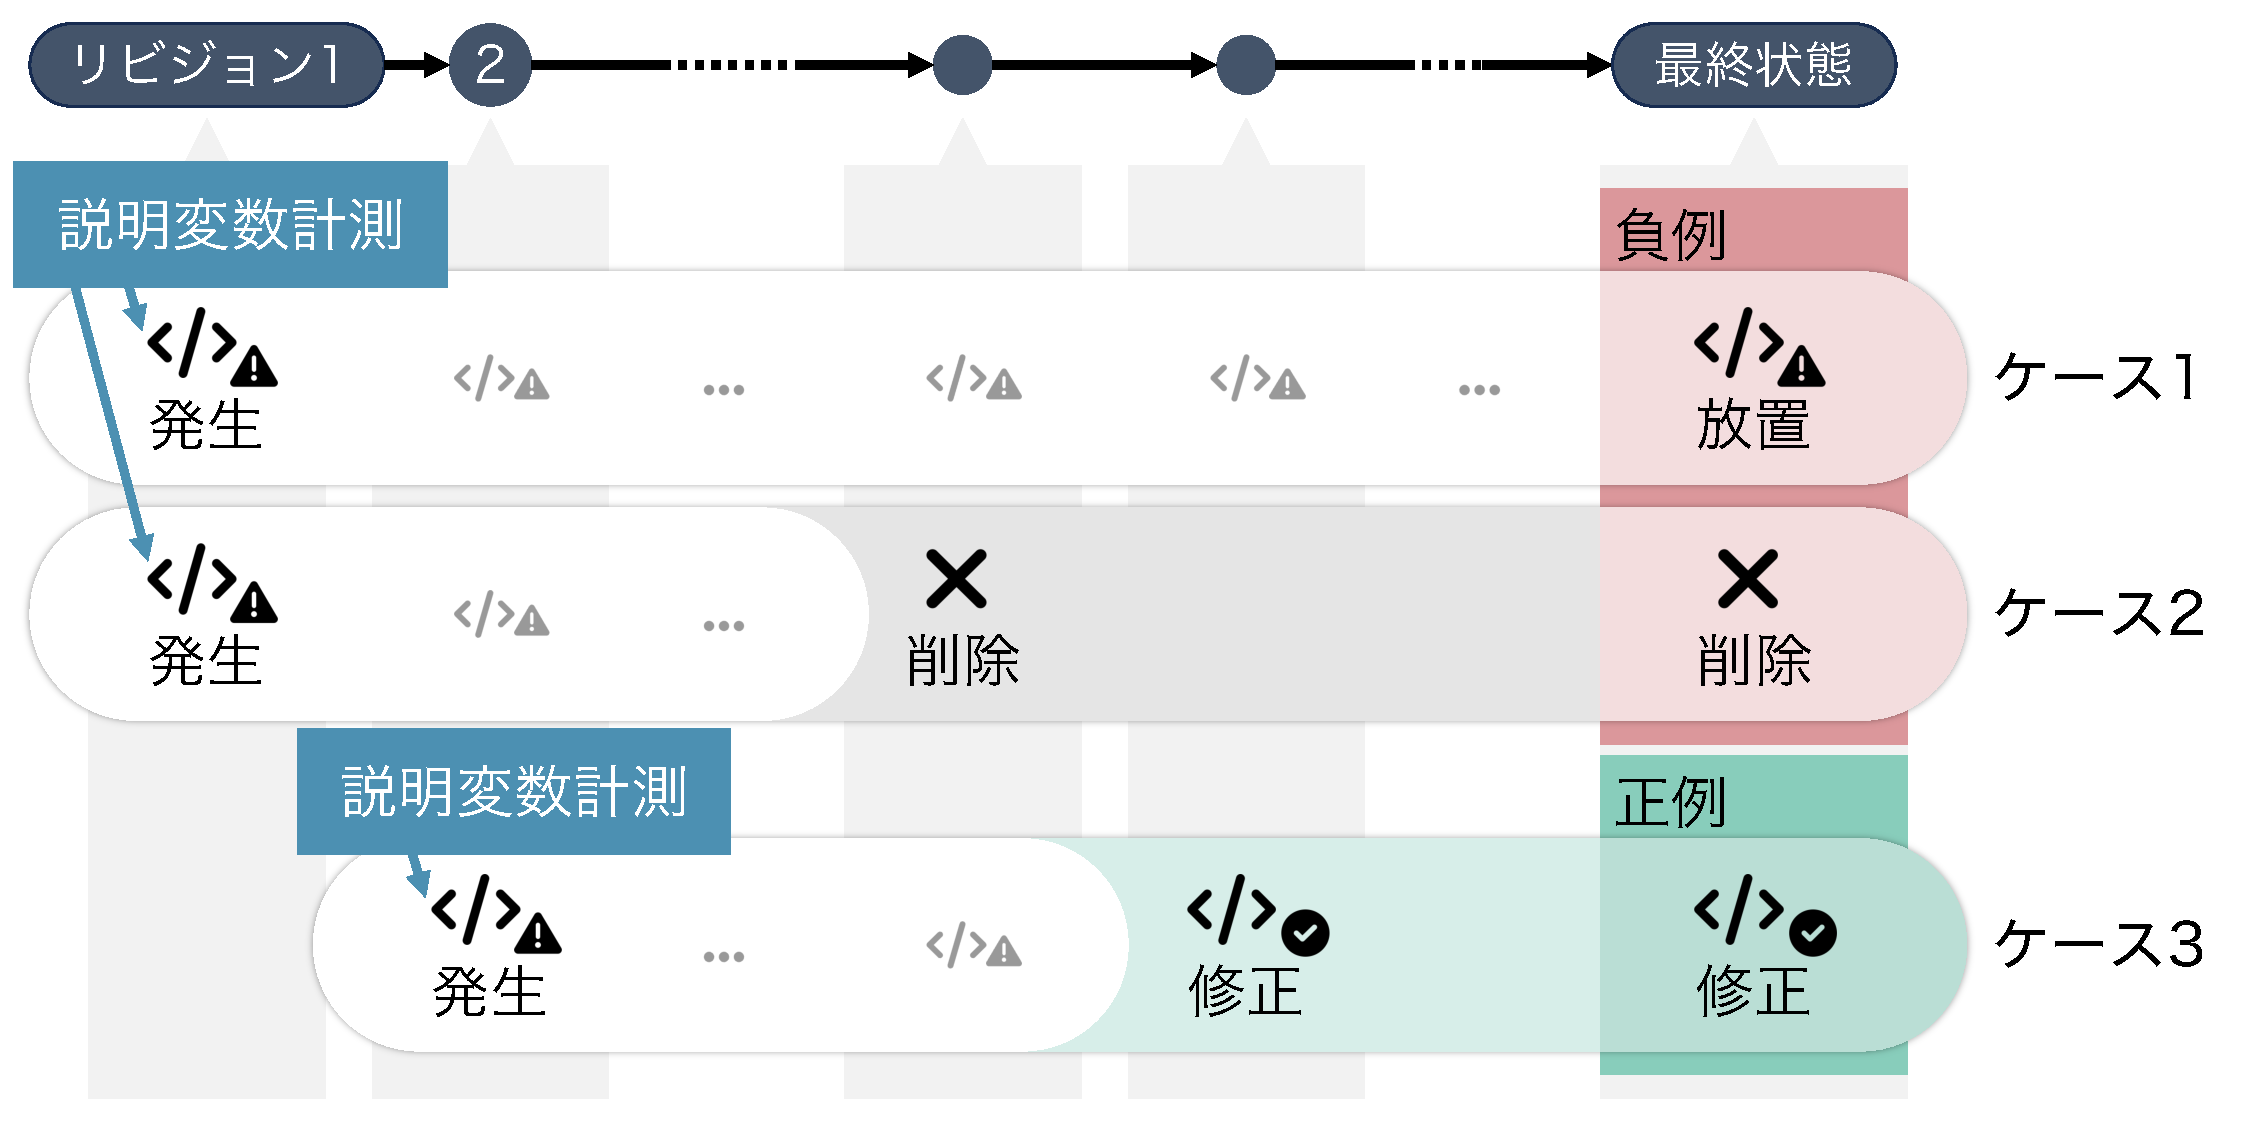
\includegraphics[width=1.0\linewidth]{Kameoka_fig/kameoka_fig2.pdf}
	\caption{説明変数と目的変数の計測方法}
	\label{fig:mokutekihensu}
\end{figure}
%-------------------------

図\ref{fig:mokutekihensu}は,本研究における説明変数と目的変数の計測位置と,計測方法を示す.本研究では,開発履歴から静的解析ツールによって初めて違反が検出された場所を説明変数の計測地点とし,最終状態において,各違反が修正されたか否かを計測することによって目的変数を計測する.
各事例について詳しく説明すると,最初の事例は,リビジョン1で発生した違反が修正されずに最終リビジョンまで放置された状況を表している.2つ目の事例は,発生した違反が途中状態で削除された場合を示している,最初の事例と2つ目の事例は発生した規約違反が修正されていないため負例として計測する.3つ目の事例は,発生した違反が途中状態において修正された場合を示しており,最終状態において正例として計測する.

目的変数の計測について各事例ごとにまとめたものが表\ref{tab:pos_neg}である.すべての計測したコーディング規約違反は表の3種類に分類され,目的変数を計測し,各違反の発生地点において説明変数を計測する.


%-----------------------------------prev
% 本研究では,分析対象期間中のコミットにおいて変更されたPython言語で記述されたソースコード全てに静的解析ツールを実行する.特定のソースコード断片において初めて規約違反が検出されたコミットを,修正を要するか否かを判定する予測時点とし,説明変数を計測する.

% 図\ref{fig:mokutekihensu}は,説明変数と目的変数の計測事例を示す.この例では,コーディング規約への違反が3箇所で検出され,上2つはリビジョン1で発生し,下の1つはリビジョン2で発生しており,それぞれのリビジョンにおいて説明変数を計測する.説明変数の計測地点において,コーディング規約に違反するコード断片を含むソースコードファイルの関数,クラス,モジュールに対して特徴量をテクマトリックス株式会社が開発する静的解析ツールUnderstand\footnote{Understand: \url{https://www.techmatrix.co.jp/product/understand/}}を用いて計測する.説明変数は,ソースコードの特徴量であるコード行数,コメント行数,循環的複雑度,ネストの深さの最大値など含むソースコードに関する特徴量43種類に,コーディング規約の違反検出時に得られる違反箇所のコード行数1種類,規約違反IDをOne-hotベクトル化した1種類の,合計45種類の特徴量を使用する.
%-----------------------------------




% \section{目的変数の計測方法}

% 本研究では,分析対象期間中に修正されるか否かを目的変数とする.分析対象期間中に修正された規約違反のコード断片と修正されないままの規約違反含むコード断片は表\ref{tab:pos_neg}に示すように正例と負例の2クラスに分類する.

%----------------------
\begin{table}[t]
    \centering
    \caption{正例と負例の分類}
    \label{tab:pos_neg}
    \scalebox{1}{
    \begin{tabular}{l|l}
         \hline
            分類 & 説明\\ \hline
            負例 & コーディング規約の違反が放置されているコード断片\\
            負例 & コーディング規約に違反していたコード断片が削除された\\
            正例 & コーディング規約に違反していたコード断片が修正された\\
         \hline
    \end{tabular}
    }
\end{table}
%-----------------------

\section{コーディング規約に違反しているコード断片のクラスタリング}


提案手法(クラスタリングあり)において,説明変数の特徴量が類似しているコード断片をクラスタリングし,各クラスタごとに予測モデルを構築する.クラスタリングには,クラスタ間の類似度を計測するため階層的クラスタリングを用いる.階層的クラスタリングには,連結法としてWard法を用い,距離の測定にはユークリッド距離を用いる.本研究ではクラスタ数を10とした場合における結果を用いて評価を行う.クラスタ数を変化させることによって予測精度が変化することが考えられるが,本研究では予測結果についてい従来手法との差分を見たいため,クラスタ数を10のみの場合で検証している.

%-----------------------------------prev
% 本研究では,説明変数の特徴量が類似する規約違反しているコード断片をクラスタリングした後に,各クラスタに分類されたコード断片の学習データを用いてモデルを構築する.クラスタリングには,クラスタ間の類似度を確認するため階層的クラスタリングを用いる.階層的クラスタリングにおける,クラスタ間の距離はユークリッド距離を用い,クラスタの連結法にはWard法を用いる.本研究では検証に10プロジェクトの開発履歴を使用するため,クラスタ数を10とする.階層クラスタリングによって,従来手法で予測できなかったコード断片を分析する.
%-----------------------------------

\section{機械学習モデルの構築と評価}

本研究で利用する予測モデルは,機械学習の予測手法として頻繁に利用されるロジスティック回帰,ランダムフォレスト,SVMの3種類の手法を用いて予測モデルの構築を行う.コーディング規約違反の修正に関するデータは,違反が修正された正例が少なく,修正されない負例が多い不均衡なデータであることが多いため,各予測モデルを構築するためのPythonパッケージに用意されているオプションであるclass\_weightsを用いることによって,2クラスデータに重みづけを行う.また,学習の反復回数を定めるイテレーション回数を10,000に設定する.

構築した各予測モデルの評価には,従来研究でも用いられていた適合率,再現率,F1値を使用した.機械学習モデルの予測結果は以下の4種類に分類され,分類結果から各評価指標の値を算出する.

%-----------------------------------prev
% 予測モデルの構築には,
% Ruthruffらの従来研究と同様にロジスティック回帰モデルを用いる\cite{JyuraiPre}.本研究で取り扱うコーディング規約に違反しているコード断片は,修正されないままのコード断片が多数含まれる不均衡なデータとなっている.したがって,本研究ではロジスティック回帰分析にはPythonパッケージであるsklearnのlinear\_model.LogisticRegression\footnote{https://scikit-learn.org/stable/modules/generated/sklearn.linear\_model.LogisticRegression.html}を使用し,パッケージのオプションclass\_weightsを使用することで2クラスデータの分類に重み付けし,不均衡による問題を解決する.また,ロジスティック回帰モデルの学習を行う際にイテレーションの最大値を10,000回に設定する.

% 予測モデルの予測性能を評価する指標として,従来研究で用いられている適合率,再現率,F1値を使用する.機械学習モデルの予測結果は次の4つに分類することができ,分類結果に基づき各評価指標を算出する.
%-----------------------------------prev

\begin{itemize}
\item True Positive(TP): 修正された規約違反に対して,修正されると正しく予測するケース
\item False Positive(FP): 放置された規約違反に対して,修正されると誤って予測するケース
\item True Negative(TN):放置された規約違反に対して,放置されると正しく予測するケース
\item False Negative(FN):修正された規約違反に対して,放置されると誤って予測するケース
\end{itemize}

\chapter{評価実験}\label{chap:result}

\section{データセット}

\begin{figure}[tbp]
	\centering
	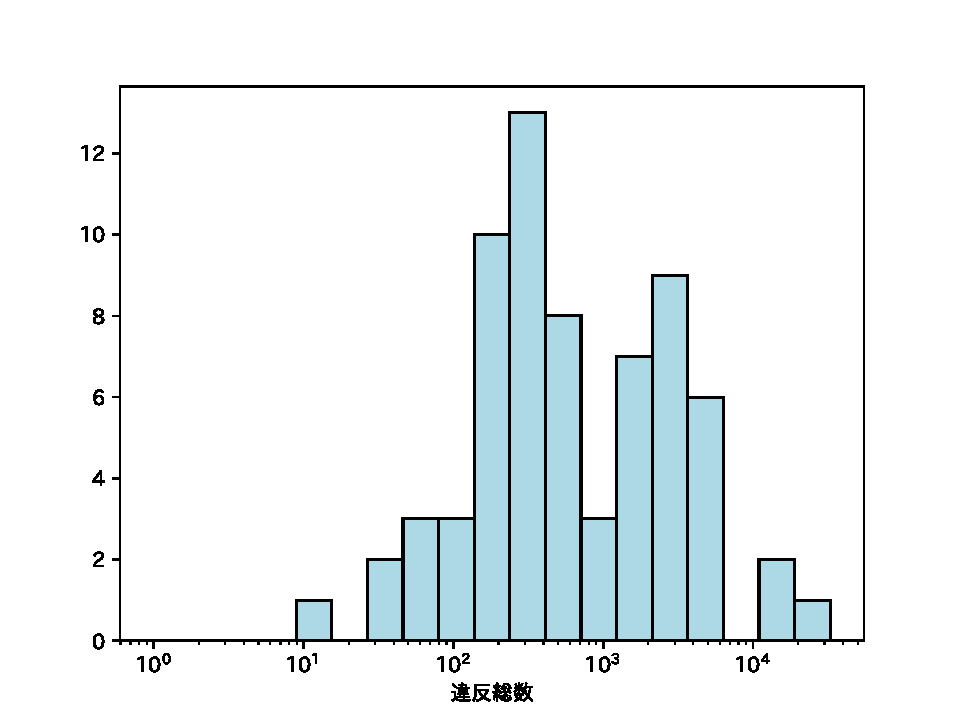
\includegraphics[width=0.7\linewidth]{Kameoka_fig/dataset_hist.pdf}
	\caption{データセットに含まれるプロジェクトごとの違反総数の箱ひげ図}
	\label{fig:dataset}
\end{figure}

% \begin{table*}[t]
%     \centering
%     \caption{分析対象プロジェクトの統計量(総違反数で昇順に記載)}
%     \label{datasetTB}
%     \scalebox{1.0}{
%     \begin{tabular}{l|r|r|r|r|r}
%          \hline
%          \multirow{2}{*}{プロジェクト名} & \multirow{2}{*}{対象リビジョン数} & \multicolumn{1}{c|}{違反修正数} & \multicolumn{1}{c|}{違反放置数}& \multicolumn{1}{c|}{\multirow{2}{*}{総違反数}} & \multicolumn{1}{c}{\multirow{2}{*}{違反修正率}} \\ 
%                       &               &\multicolumn{1}{c|}{(正例)} & \multicolumn{1}{c|}{(負例)} &&\\ \hline
%          \hline %
% python-bugzilla & 243 & 189 & 183 & 372 & 51\%\\
% python-cloudant & 657 & 269 & 1,299 & 1,568 & 17\%\\
% pynput & 507 & 431 & 3,595 & 4,026 & 11\%\\
% pyscard & 380 & 681 & 2,705 & 3,386 & 20\%\\
% howdoi & 593 & 721 & 434 & 1,155 & 62\%\\
% hickle & 245 & 920 & 1,293 & 2,213 & 42\%\\
% transitions & 496 & 1,182 & 2,620 & 3,802 & 31\%\\
% OWSLib & 422 & 1,547 & 3,080 & 4,627 & 33\%\\
% schema\_salad & 564 & 1,990 & 3,009 & 4,999 & 40\%\\
% schematics & 524 & 6,950 & 4,829 & 11,779 & 59\%\\
%          \hline
%     \end{tabular}
%     }
% \end{table*}

%--------------------
% \begin{table*}[t]
%     \centering
%     \caption{予測結果}
%     \label{PrevPrediction}
%     \begin{tabular}{l|ccc|ccc|ccc}
%          \hline
%          \multirow{3}{*}{プロジェクト名}&\multicolumn{3}{c|}{\multirow{2}{*}{従来手法}} & \multicolumn{3}{c|}{提案手法} & \multicolumn{3}{c}{提案手法}\\
%          &\multicolumn{3}{c|}{} & \multicolumn{3}{c|}{(クラスタリングなし)} & \multicolumn{3}{c}{(クラスタリングあり)}\\ \cline{2-10}
%           & 適合率 & 再現率 & F1値 & 適合率 & 再現率 & F1値 & 適合率 & 再現率 & F1値\\ \hline
%          \hline %
%             python-bugzilla & 0.54 & 0.13 & 0.21 & \textbf{\underline{0.69}} & \textbf{\underline{0.64}} & \textbf{\underline{0.67}} & 0.63 & 0.23 & 0.33\\
%             python-cloudant & \textbf{\underline{0.77}} & \textbf{\underline{0.81}} & \textbf{\underline{0.79}} & 0.17 & 0.17 & 0.17 & 0.65 & 0.32 & 0.43\\
%             pynput & 0.41 & \textbf{\underline{0.94}} & 0.58 & 0.42 & 0.71 & 0.53 & \textbf{\underline{0.57}} & 0.65 & \textbf{\underline{0.61}}\\
%             pyscard & \textbf{\underline{0.29}} & \textbf{\underline{0.91}} & \textbf{\underline{0.44}} & 0.18 & 0.89 & 0.30 & 0.12 & 0.41 & 0.18\\
%             howdoi & 0.92 & \textbf{\underline{0.96}} & \textbf{\underline{0.94}} & \textbf{\underline{0.93}} & 0.59 & 0.72 & \textbf{\underline{0.93}} & 0.51 & 0.66\\
%             hickle & 0.33 & \textbf{\underline{0.73}} & 0.45 & 0.36 & 0.66 & \textbf{\underline{0.47}} & \textbf{\underline{0.41}} & 0.47 & 0.44\\
%             transitions & \textbf{\underline{0.80}} & \textbf{\underline{0.87}} & \textbf{\underline{0.83}} & 0.68 & 0.50 & 0.57 & 0.68 & 0.21 & 0.32\\
%             OWSLib & \textbf{\underline{0.84}} & 0.86 & \textbf{\underline{0.85}} & 0.76 & \textbf{\underline{0.92}} & 0.83 & 0.83 & 0.88 & \textbf{\underline{0.85}}\\
%             schema\_salad & \textbf{\underline{0.52}} & \textbf{\underline{0.66}} & \textbf{\underline{0.58}} & 0.21 & 0.52 & 0.30 & 0.15 & 0.21 & 0.17\\
%             schematics & \textbf{\underline{0.30}} & 0.79 & \textbf{\underline{0.44}} & 0.26 & \textbf{\underline{0.94}} & 0.41 & 0.27 & 0.84 & 0.40\\
%     \hline
%     \end{tabular}
% \end{table*}
%--------------------

% \begin{table*}[t]
%     \centering
%     \caption{従来手法の予測結果分析}
%     \label{PrevPredictionCrustering}
%     \scalebox{0.67}{
%     \begin{tabular}{l|c|c|c|c|c|c|c|c|c|c}
%          \hline
%          プロジェクト名 & cluster 1 & cluster 2 & cluster 3 & cluster 4 & cluster 5 & cluster 6 & cluster 7 & cluster 8 & cluster 9 & cluster 10\\ \hline
%          \hline %
%          python-bugzilla & \textbf{\underline{0.67}}* & -- & 0.33* & -- & 0.13* & -- & --* & -- & -- & -- \\ \hline
%          python-cloudant & \textbf{\underline{0.95}}* & -- & \textbf{\underline{0.89}}* & -- & 0.89* & -- & \textbf{\underline{0.97}}* & -- & -- & -- \\ \hline
%          pynput & 0.70* & -- & 0.35* & -- & -- & -- & -- & -- & -- & \textbf{\underline{1.00}}* \\ \hline
%          pyscard & \textbf{\underline{0.76}}* & \textbf{\underline{1.00}}* & \textbf{\underline{0.78}}* & -- & -- & --* & -- & -- & \textbf{\underline{1.00}}* & -- \\ \hline
%          howdoi & 0.57* & -- & \textbf{\underline{0.91}}* & -- & -- & -- & -- & -- & -- & -- \\ \hline
%          hickle & -- & -- & 0.51* & -- & -- & -- & -- & -- & -- & -- \\ \hline
%          transitions & \textbf{\underline{0.82}}* & -- & \textbf{\underline{0.86}}* & -- & --* & -- & \textbf{\underline{0.80}}* & -- & -- & -- \\ \hline
%          OWSLib & 0.94* & \textbf{\underline{1.00}}* & \textbf{\underline{0.80}}* & -- & \textbf{\underline{1.00}}* & -- & \textbf{\underline{0.87}}* & \textbf{\underline{1.00}}* & -- & -- \\ \hline
%          schema\_salad & \textbf{\underline{0.72}}* & -- & \textbf{\underline{0.86}}* & 0.62* & \textbf{\underline{0.92}}* & -- & 0.26* & -- & -- & -- \\ \hline
%          schematics & \textbf{\underline{0.47}}* & -- & \textbf{\underline{0.47}}* & -- & -- & -- & \textbf{\underline{0.56}}* & -- & -- & -- \\
%          \hline
%     \end{tabular}
%     }

% \vspace{1mm}

%     \centering
%     \vspace{1mm}
%     \caption{提案手法(クラスタリングなし)の予測結果分析}
%     \label{MergePredictionCrustering}
%     \scalebox{0.67}{
%     \begin{tabular}{l|c|c|c|c|c|c|c|c|c|c}
%          \hline
%          プロジェクト名 & cluster 1 & cluster 2 & cluster 3 & cluster 4 & cluster 5 & cluster 6 & cluster 7 & cluster 8 & cluster 9 & cluster 10\\ \hline
%          \hline %
%          python-bugzilla & \textbf{\underline{0.67}}* & -- & \textbf{\underline{0.42}}* & -- & \textbf{\underline{1.00}}* & -- & --* & -- & -- & -- \\ \hline
%          python-cloudant & 0.71* & -- & 0.72* & -- & 0.73* & -- & 0.73* & -- & -- & -- \\ \hline
%          pynput & 0.57* & -- & 0.56* & -- & -- & -- & -- & -- & -- & \textbf{\underline{1.00}}* \\ \hline
%          pyscard & 0.58* & \textbf{\underline{1.00}}* & 0.60* & -- & -- & --* & -- & -- & \textbf{\underline{1.00}}* & -- \\ \hline
%          howdoi & 0.57* & -- & 0.62* & -- & -- & -- & -- & -- & -- & -- \\ \hline
%          hickle & -- & -- & 0.59* & -- & -- & -- & -- & -- & -- & -- \\ \hline
%          transitions & 0.69* & -- & 0.60* & -- & --* & -- & 0.52* & -- & -- & -- \\ \hline
%          OWSLib & 0.91* & \textbf{\underline{1.00}}* & 0.75* & -- & \textbf{\underline{1.00}}* & -- & 0.85* & \textbf{\underline{1.00}}* & -- & -- \\ \hline
%          schema\_salad & 0.54* & -- & 0.09* & \textbf{\underline{0.78}}* & 0.03* & -- & \textbf{\underline{0.78}}* & -- & -- & -- \\ \hline
%          schematics & 0.20* & -- & 0.34* & -- & -- & -- & 0.45* & -- & -- & -- \\
%          \hline
%     \end{tabular}
%     }

    
% \vspace{1mm}
%     \centering
%     \vspace{1mm}
%     \caption{提案手法(クラスタリングあり)の予測結果分析}
%     \label{AproPredictionCrustering}
%     \scalebox{0.67}{
%     \begin{tabular}{l|c|c|c|c|c|c|c|c|c|c}
%          \hline
%          プロジェクト名 & cluster 1 & cluster 2 & cluster 3 & cluster 4 & cluster 5 & cluster 6 & cluster 7 & cluster 8 & cluster 9 & cluster 10\\ \hline
%          \hline %
%          python-bugzilla & \textbf{\underline{0.67}}* & -- & 0.37* & -- & 0.27* & -- & --* & -- & -- & -- \\ \hline
%          python-cloudant & 0.90* & -- & 0.77* & -- & \textbf{\underline{0.91}}* & -- & 0.73* & -- & -- & -- \\ \hline
%          pynput & \textbf{\underline{0.80}}* & -- & \textbf{\underline{0.64}}* & -- & -- & -- & -- & -- & -- & \textbf{\underline{1.00}}* \\ \hline
%          pyscard & 0.63* & \textbf{\underline{1.00}}* & 0.64* & -- & -- & --* & -- & -- & \textbf{\underline{1.00}}* & -- \\ \hline
%          howdoi & 0.57* & -- & 0.55* & -- & -- & -- & -- & -- & -- & -- \\ \hline
%          hickle & -- & -- & \textbf{\underline{0.67}}* & -- & -- & -- & -- & -- & -- & -- \\ \hline
%          transitions & 0.61* & -- & 0.21* & -- & --* & -- & 0.53* & -- & -- & -- \\ \hline
%          OWSLib & \textbf{\underline{0.95}}* & \textbf{\underline{1.00}}* & \textbf{\underline{0.80}}* & -- & \textbf{\underline{1.00}}* & -- & 0.86* & \textbf{\underline{1.00}}* & -- & -- \\ \hline
%          schema\_salad & 0.44* & -- & 0.51* & 0.62* & 0.03* & -- & 0.22* & -- & -- & -- \\ \hline
%          schematics & 0.23* & -- & 0.42* & -- & -- & -- & 0.55* & -- & -- & -- \\
%          \hline
%     \end{tabular}
%     }

% \vspace{1mm}
%     \centering
%     \vspace{1mm}
%     \caption{各クラスタが保有するデータ数(k=10)}
%     \label{CrusteringDataNum}
%     \scalebox{0.67}{
%     \begin{tabular}{l|c|c|c|c|c|c|c|c|c|c}
%          \hline
%          プロジェクト名 & cluster 1 & cluster 2 & cluster 3 & cluster 4 & cluster 5 & cluster 6 & cluster 7 & cluster 8 & cluster 9 & cluster 10\\ \hline
%          \hline %
%          python-bugzilla & 65* & -- & 80* & -- & 65* & -- & 97* & -- & -- & -- \\ \hline
%          python-cloudant & 473* & -- & 455* & -- & 181* & -- & 145* & -- & -- & -- \\ \hline
%          pynput & 489* & -- & 299* & -- & -- & -- & -- & -- & -- & 2,432* \\ \hline
%          pyscard & 334* & 204* & 2,053* & -- & -- & 71* & -- & -- & 46* & -- \\ \hline
%          howdoi & 223* & -- & 701* & -- & -- & -- & -- & -- & -- & -- \\ \hline
%          hickle & -- & -- & 1,770* & -- & -- & -- & -- & -- & -- & -- \\ \hline
%          transitions & 1,261* & -- & 655 & -- & 417* & -- & 708* & -- & -- & -- \\ \hline
%          OWSLib & 574* & 37* & 2,443* & -- & 83 & -- & 555* & 9* & -- & -- \\ \hline
%          schema\_salad & 1,019* & -- & 1,139* & 871* & 385* & -- & 585* & -- & -- & -- \\ \hline
%          schematics & 2,959* & -- & 4,860* & -- & -- & -- & 1,604* & -- & -- & -- \\
%          \hline
%     \end{tabular}
%     }
% \end{table*}
\subsection{対象プロジェクトの選定方法}
本研究ではケーススタディとして,OSSライブラリ検索サービスであるLibraries.io\footnote{Libraries.io: \url{https://libraries.io/}}からPython言語で実装され,静的解析ツールPylintを開発に使用しており,GitHubにソフトウェア,および開発履歴を公開しているプロジェクトを対象とする.

具体的には,Librsries.ioにおいてOSSの人気度合いや活発度合いを示すSourceRankの上位1,500プロジェクトから静的解析ツールの設定ファイル(pylintrc or .pylintrc)を保有する81プロジェクトの内,取得した目的変数を学習用データと検証用データに分割した際に,どちらにも正例と負例を含む68プロジェクトを選択した.

本研究では,各分析対象プロジェクトにおいて,2018年12月から1,000日間のコミット履歴を分析対象とする.図\ref{fig:dataset}は,各プロジェクトの総コーディング規約違反数をヒストグラムで示したものである.図の横軸は対数軸になっており,違反数が100-1,000のプロジェクトが最も多い.

\subsection{対象プロジェクト・静的解析ツールの選定理由}

Python言語は,近年のLLM(大規模言語モデル)をはじめとする機械学習技術の開発・利用に頻繁に用いられている.また,Pythonはデータ分析においても充実したライブラリが存在し,その有用性が広く知られている.よって,Python言語を研究対象の言語として選択した.

利用する静的解析ツールにはPylintを利用した.Pylintを選定した理由として,Pylintは他の静的解析ツールより多くのコーディング規約が設定されていることが特徴であるからである.


\section{RQ}

\subsection{RQ1: 複数プロジェクトのデータ用いることで予測精度は向上するか?}

\begin{table}{}
    \centering
    \caption{各手法による評価指標で最も高い値で予測したプロジェクト数の一覧}
    \label{tab:gen}
    \vspace{3mm}
    \scalebox{0.75}{
        \begin{tabular}{l||p{4em}|p{4em}|p{4em}||p{4em}|p{4em}|p{4em}||p{4em}|p{4em}|p{4em}}
            \hline
            \multirow{2}{*}{手法}&\multicolumn{3}{c||}{{ロジスティック回帰}} & \multicolumn{3}{c||}{RandomForest} & \multicolumn{3}{c}{SVM}\\ \cline{2-10}
             & 適合率 & 再現率 & F1値 & 適合率 & 再現率 & F1値 & 適合率 & 再現率 & F1値\\ \hline
            従来手法 & 48 & 27 & 38 & 28 & 43 & 37 & 36 & 24 & 28 \\
            提案手法(クラスタリングなし) & 12 & 40 & 18 & 27 & 35 & 23 & 17 & 25 & 18 \\
            提案手法(クラスタリングあり) & 20 & 22 & 19  & 28 & 24 & 16 & 24 & 36 & 26 \\ \hline
            重複数 & 12 & 21 & 7 & 15 & 34 & 8 & 9 & 17 & 4 \\
        \end{tabular}
    }
\end{table}

\begin{table}{}
    \centering
    \caption{ロジスティック回帰モデルでの予測結果(総違反数の上下5件ずつを掲載)}
    \label{tab:logistic}
    \vspace{3mm}
    \scalebox{0.75}{
        \begin{tabular}{l||p{4em}|p{4em}|p{4em}||p{4em}|p{4em}|p{4em}||p{4em}|p{4em}|p{4em}}
            \hline
            \multirow{3}{*}{プロジェクト名}&\multicolumn{3}{c||}{\multirow{2}{*}{従来手法}} & \multicolumn{3}{c||}{提案手法} & \multicolumn{3}{c}{提案手法}\\
            &\multicolumn{3}{c||}{} & \multicolumn{3}{c||}{(クラスタリングなし)} & \multicolumn{3}{c}{(クラスタリングあり)}\\ \cline{2-10}
            & 適合率 & 再現率 & F1値 & 適合率 & 再現率 & F1値 & 適合率 & 再現率 & F1値 \\ \hline
            sockeye & 0.53 & 0.81 & 0.64 & 0.35 & 0.56 & 0.43 & 0.49 & 0.67 & 0.57 \\
            coretools & 0.04 & 0.63 & 0.07 & 0.02 & 0.88 & 0.04 & 0.03 & 0.83 & 0.05 \\
            howdoi & 0.64 & 0.99 & 0.78 & 0.12 & 0.33 & 0.17 & 0.22 & 0.25 & 0.23 \\
            schema\_salad & 0.55 & 0.27 & 0.37 & 0.51 & 0.64 & 0.56 & 0.55 & 0.54 & 0.54 \\
            serverless-application-model & 0.76 & 0.45 & 0.57 & 0.55 & 0.83 & 0.66 & 0.64 & 0.83 & 0.72 \\
            \hline \hline
            implicit & 1.00 & 0.44 & 0.62 & 0.70 & 0.78 & 0.74 & 1.00 & 0.11 & 0.20 \\
            python-sshpubkeys & 0.64 & 1.00 & 0.78 & 0.71 & 0.71 & 0.71 & 0.64 & 1.00 & 0.78 \\
            munch & 0.43 & 1.00 & 0.60 & 0.33 & 0.33 & 0.33 & 0.38 & 1.00 & 0.55 \\
            python-resize-image & 0.14 & 1.00 & 0.25 & 0.17 & 1.00 & 0.29 & 0.20 & 1.00 & 0.33 \\
            queuelib & nan & 0.00 & nan & 0.33 & 1.00 & 0.50 & 0.33 & 1.00 & 0.50 \\
        \end{tabular}
    }
\end{table}

\begin{table}{}
    \centering
    \caption{RandomForestモデルでの予測結果(総違反数の上下5件ずつを掲載)}
    \label{tab:RandomForest}
    \vspace{3mm}
    \scalebox{0.75}{
        \begin{tabular}{l||p{4em}|p{4em}|p{4em}||p{4em}|p{4em}|p{4em}||p{4em}|p{4em}|p{4em}}
            \hline
            \multirow{3}{*}{プロジェクト名}&\multicolumn{3}{c||}{\multirow{2}{*}{従来手法}} & \multicolumn{3}{c||}{提案手法} & \multicolumn{3}{c}{提案手法}\\
            &\multicolumn{3}{c||}{} & \multicolumn{3}{c||}{(クラスタリングなし)} & \multicolumn{3}{c}{(クラスタリングあり)}\\ \cline{2-10}
            & 適合率 & 再現率 & F1値 & 適合率 & 再現率 & F1値 & 適合率 & 再現率 & F1値 \\ \hline
            sockeye & 0.75 & 0.83 & 0.79 & 0.76 & 0.79 & 0.78 & 0.76 & 0.80 & 0.78 \\
            coretools & 0.14 & 0.24 & 0.18 & 0.04 & 0.41 & 0.08 & 0.04 & 0.37 & 0.07 \\
            howdoi & 0.78 & 0.99 & 0.87 & 0.07 & 0.99 & 0.13 & 0.07 & 0.99 & 0.13 \\
            schema\_salad & 0.66 & 0.58 & 0.62 & 0.58 & 0.31 & 0.41 & 0.46 & 0.21 & 0.29 \\
            serverless-application-model & 0.72 & 0.27 & 0.39 & 0.70 & 0.23 & 0.34 & 0.63 & 0.24 & 0.35 \\
            \hline \hline
            implicit & 0.75 & 1.00 & 0.86 & 1.00 & 0.44 & 0.62 & 1.00 & 0.44 & 0.62 \\
            python-sshpubkeys & 0.64 & 1.00 & 0.78 & 0.71 & 0.71 & 0.71 & 0.67 & 0.29 & 0.40 \\
            munch & nan & 0.00 & nan & nan & 0.00 & nan & nan & 0.00 & nan \\
            python-resize-image & 0.14 & 1.00 & 0.25 & 0.14 & 1.00 & 0.25 & 0.17 & 1.00 & 0.29 \\
            queuelib & nan & 0.00 & nan & nan & 0.00 & nan & nan & 0.00 & nan \\
        \end{tabular}
    }
\end{table}

\begin{table}{}
    \centering
    \caption{SVMモデルでの予測結果(総違反数の上下5件ずつを掲載)}
    \label{tab:SVM}
    \vspace{3mm}
    \scalebox{0.75}{
        \begin{tabular}{l||p{4em}|p{4em}|p{4em}||p{4em}|p{4em}|p{4em}||p{4em}|p{4em}|p{4em}}
            \hline
            \multirow{3}{*}{プロジェクト名}&\multicolumn{3}{c||}{\multirow{2}{*}{従来手法}} & \multicolumn{3}{c||}{提案手法} & \multicolumn{3}{c}{提案手法}\\
            &\multicolumn{3}{c||}{} & \multicolumn{3}{c||}{(クラスタリングなし)} & \multicolumn{3}{c}{(クラスタリングあり)}\\ \cline{2-10}
            & 適合率 & 再現率 & F1値 & 適合率 & 再現率 & F1値 & 適合率 & 再現率 & F1値 \\ \hline
            sockeye & 0.47 & 0.71 & 0.57 & 0.3 & 0.48 & 0.37 & 0.5 & 0.6 & 0.54 \\
            coretools & 0.02 & 0.68 & 0.04 & 0.02 & 0.49 & 0.03 & 0.03 & 0.88 & 0.06 \\
            howdoi & 0.05 & 0.99 & 0.1 & 0.05 & 0.21 & 0.08 & 0.15 & 0.2 & 0.17 \\
            schema\_salad & 0.48 & 0.43 & 0.45 & 0.51 & 0.58 & 0.54 & 0.51 & 0.66 & 0.57 \\
            serverless-application-model & 0.69 & 0.56 & 0.62 & 0.47 & 0.37 & 0.41 & 0.59 & 0.77 & 0.67 \\
            \hline \hline
            implicit & 1 & 0.44 & 0.62 & 0.57 & 0.44 & 0.5 & 1 & 0.22 & 0.36 \\
            python-sshpubkeys & 0.64 & 1 & 0.78 & nan & 0 & nan & 0.64 & 1 & 0.78 \\
            munch & nan & 0 & nan & 1 & 0.33 & 0.5 & 1 & 0.33 & 0.5 \\
            python-resize-image & 0.14 & 1 & 0.25 & 0.5 & 1 & 0.67 & 0.2 & 1 & 0.33 \\
            queuelib & nan & 0 & nan & nan & 0 & nan & 0.33 & 1 & 0.5 \\
        \end{tabular}
    }
\end{table}

\begin{table}{}
    \centering
    \caption{ロジスティック回帰モデルで再現率とF1値が向上した予測結果}
    \label{tab:log-super}
    \vspace{3mm}
    \scalebox{0.75}{
        \begin{tabular}{l||p{4em}|p{4em}|p{4em}||p{4em}|p{4em}|p{4em}||p{4em}|p{4em}|p{4em}}
            \hline
            \multirow{3}{*}{プロジェクト名}&\multicolumn{3}{c||}{\multirow{2}{*}{従来手法}} & \multicolumn{3}{c||}{提案手法} & \multicolumn{3}{c}{提案手法}\\
            &\multicolumn{3}{c||}{} & \multicolumn{3}{c||}{(クラスタリングなし)} & \multicolumn{3}{c}{(クラスタリングあり)}\\ \cline{2-10}
            & 適合率 & 再現率 & F1値 & 適合率 & 再現率 & F1値 & 適合率 & 再現率 & F1値 \\ \hline
            schema\_salad & 0.55 & 0.27 & 0.37 & 0.51 & 0.64 & 0.56 & 0.55 & 0.54 & 0.54 \\
            pyphi & 0.66 & 0.57 & 0.61 & 0.68 & 0.74 & 0.71 & 0.59 & 0.61 & 0.6 \\
            serverless-application-model & 0.76 & 0.45 & 0.57 & 0.55 & 0.83 & 0.66 & 0.64 & 0.83 & 0.72 \\
            behave & 0.18 & 0.48 & 0.26 & 0.15 & 0.65 & 0.25 & 0.21 & 0.67 & 0.32 \\
        \end{tabular}
    }
\end{table}


従来手法と提案手法2種の予測結果を評価した概要を表\ref{tab:gen}に示す.
それぞれの手法とモデル構築手法のF1値を比較すると,従来手法が最多の最大値をとっていることがわかる.
しかし,提案手法によって再現率が改善されているプロジェクトが多い.特にロジスティック回帰モデルの再現率が最大値のプロジェクト数は従来手法で27であり,提案手法(クラスタリングなし)では40に増加している.再現率が向上した理由として,提案手法は複数プロジェクトのデータを学習に用いているため,単一プロジェクトでは,修正されることが学習できなかったことが,学習データを拡張したことによって予測が可能になったと考えられる.対して,データセットを拡張したことによって,正例と予測する範囲が広がったため,従来手法で真陰性として予測できていたものを偽陽性として予測したため,提案手法によって適合率が低下したと考えられる.

表\ref{tab:logistic} - \ref{tab:SVM}は従来手法と提案手法2種の予測結果の値を示す.
各表はプロジェクトに対して従来手法,提案手法(クラスタリングなし),提案手法(クラスタリングあり)による予測結果の適合率,再現率,F1値を算出したものである.
結果として掲載しているプロジェクトは,各プロジェクトで検出された違反総数でソートした上位と下位から5プロジェクトを抽出したものである.
表\ref{tab:logistic}, \ref{tab:RandomForest}中に含まれる`nan'は予測結果をすべて負例として予測し,適合率とF1値を計算することができなかったため`nan'としている.
予測結果の再現率が向上したプロジェクトは,違反総数で降順にソートした場合,20プロジェクト目以降で頻繁に見られた.このことから,学習データが十分に集まるプロジェクトでは従来手法のような単一のプロジェクトの開発履歴を学習し,プロジェクトごとの修正の特性を考慮した予測を行う方が高い精度で修正予測ができると示唆される.

\subsection{RQ2: 提案手法によって従来では予測できなかった修正予測ができるか?}\label{RQ2}

RQ1の結果から,提案手法によってデータセットを拡張したことによって修正されると予測されたものが増加し,再現率が向上し,適合率が低下したことが示唆された.
本章では,従来手法と提案手法の具体的な予測結果について分析を行う.分析を行う対象として,RQ1において提案手法によって予測精度が向上したプロジェクトから選択して分析を行う.

表\ref{tab:log-super}はロジスティック回帰モデルを用いた提案手法によって再現率とF1値が共に向上したプロジェクトの予測結果を抜粋したものである.ロジスティック回帰モデルの結果を抜粋した理由としては,3種類のモデルの中で提案手法によって最も精度の改善が見られたからである.1, 2行目の`schema\_salad'と`pyphi'プロジェクトは提案手法(クラスタリングなし)によって向上し,3, 4行目の`serverless-application-model'と`behave'プロジェクトは提案手法(クラスタリングあり)によって向上した結果である.表\ref{tab:log-super}に記載した提案手法によって予測精度が向上した4プロジェクトにおける修正予測結果について分析を行う.



\subsubsection{分析1 提案手法によって予測可能になったものとは?}

\subsubsection{分析2 提案手法によって余剰に正例として予測したものとは?}


\chapter{考察}\label{chap:consideration}
\section{RQ1の結果からなぜ提案手法によって再現率が向上したのか}
\section{RQ1の結果からなぜ提案手法によって再現率が向上したのか}


\chapter{妥当性への脅威}\label{chap:heuristic}
\section{内的妥当性}

本研究で利用したデータセットは,プロジェクトごとの開発履歴の期間は統一して収集しているが,複数プロジェクトを結合して学習した場合には予測地点では得られない他プロジェクトの未来のデータを学習している.複数プロジェクトのデータを学習し,予測する際にも時系列を考慮することは今後の課題である.

目的変数の計測において,規約違反しているコードが削除された場合は,修正されたわけではないため本研究では負例として扱っている.しかし,コーディング規約違反の中には該当部分を削除することによっても解消するものがあるため,本来正例として扱うべきケースを負例として計測してしまっていることがある.

%-----------------------------------prev
% 提案手法または,クラスタリングを行わずに複数プロジェクトの開発履歴を統合することによって学習データを拡大した.各プロジェクトにおいてデータセットの分割では時系列を考慮しているが,プロジェクト間では時系列の順序を考慮していない.プロジェクト間においても時系列を考慮した学習データを作成することは今後の課題である.
%-----------------------------------

\section{外的妥当性}

本研究ではケーススタディとしてPython言語を主な開発言語としたプロジェクト68件の開発履歴を収集して検証を行ったが,データサイズをさらに拡張した場合,予測精度に影響が出ることが示唆される.

%-----------------------------------prev
% 本研究ではケーススタディとして10プロジェクト分のデータを学習し予測を行ったが,データセットを拡張することによって正例が増加し予測性能が向上することも示唆されるが,一方で,学習データ増加により各クラスタで作成したモデルが汎化することも考えられる.今後は,プロジェクト数,クラスタ数の適性についても検討する.
%-----------------------------------

\chapter{おわりに}\label{chap:end}

\todo{コピペしたまま}

%-----------------------------------prev
% 本研究では,静的解析ツールによって大量に検出されるコーディング規約に違反しているコード断片の中から,優先して修正すべき違反の予測を,複数プロジェクトのデータを結合し,類似性に基づいてクラスタリングしたデータセットを用いることによる予測精度への影響を明らかにした.検証の結果,予測精度だけを見れば,単一プロジェクトのデータだけを用いて学習するほうが予測に効果的であった.今後は考察でも述べたように,多くのデータを保有するクラスタをさらに分割することや,データ数の少ないクラスタ同士の結合によって修正予測精度の向上を目指し,複数プロジェクトのデータを機械学習モデルに学習させる手法の有効性を明らかにする.
%-----------------------------------

\chapter*{謝辞}\label{chap:thanks}

研究活動に取り組むにあたって多くの方々に御指導,御協力を賜りました.ここに御世話 になった方々への感謝の意を記させていただきます.はじめに,指導教員である和歌山大学システム工学部伊原彰紀准教授に対し,厚く御礼申し上げます.研究室に配属して以来,研究方針についての相談,論文執筆,発表資料制作など多くの時間を割いて御指導をしていただきました.特に学会発表の際には,夜分にもかかわらずご対応いただき,無事発表を行うことができました.先生の御尽力に敬意を 表し,心より感謝いたします.

次に,和歌山大学システム工学研究科を修了された南雄太氏並びに,和歌山大学システム工学研究科大森楓己氏には,研究において多くの御指導,御協力,御助言をしていただきました.お忙しい中,研究内容の相談や,論文執筆,実装方法についての支援だけでなく,発表資料制作についても多大なるご協力を賜りました.心より感謝いたします.

また,和歌山大学ソーシャルソフトウェア工学研究室の方々には,研究に関する客観的な御意見や御指摘を常日頃からかず多くいただきました.研究活動の他にも,研究室での生活においても,大変お世話になりました.特に切磋琢磨し互いに高めあうことができた同期がいたことが,研究生活において大きな支えとなりました.心より感謝いたします.

%-----------------------------------prev
% 研究を進めるにあたり多くの方々に,御指導,御協力,御支援を賜りました.ここに御世話 になった方々への感謝の意を記させていただきます.はじめに,指導教員である和歌山大学シス テム工学部伊原彰紀講師に対し,厚く御礼申し上げます.研究室配属以降,研究内容の議論,論 文執筆,発表資料制作など多くの時間を割いて御指導をしていただきました.特に,学会発表の 機会をいただいたことで,研究に対する視野を広げることができました.先生の御尽力に敬意を 表し,心より感謝いたします.

% 次に,和歌山大学システム工学研究科才木一也氏には,研究において多くの御指導,御協力,御 助言をしていただきました.研究内容の議論のため,お忙しい中,平時よりお気遣いいただきま した.特に,分析手法や実装方法,発表練習など多くの御指導を賜りました.心より感謝いたし ます.

% また,和歌山大学ソーシャルソフトウェア工学研究室の方々には,研究に関する客観的な御意 見や御協力を常日頃から数多くいただきました.研究活動だけでなく,大学生活においても大変 お世話になりました.研究室の方々と交流を深めたり,切磋琢磨し合う同期がいたことは,研究 活動を進める上で支えとなりました.心より感謝いたします.最後になりましたが,日頃から暖 かく見守り,支えてくださった家族には心より感謝いたします
%-----------------------------------

%%%%%%%%%%%%%%%%%%%%%%%%%%%%%%%%%%%%%%%%%%%%%%%%%%%%%%%%%%%%%%%%%%%%%%%%

%%
%% 謝辞
%%
%% \begin{acknowledgements}
%% 感謝します.
%% \end{acknowledgements}

%%%%%%%%%%%%%%%%%%%%%%%%%%%%%%%%%%%%%%%%%%%%%%%%%%%%%%%%%%%%%%%%%%%%%%%%

%%
%% 参考文献
%%
\bibliographystyle{junsrt}
\bibliography{Kameoka}

%%%%%%%%%%%%%%%%%%%%%%%%%%%%%%%%%%%%%%%%%%%%%%%%%%%%%%%%%%%%%%%%%%%%%%%%

%%
%% 付録
%%
% \appendix
% 
% \chapter{サンプルプログラム}
% 
% プログラムリストや実行結果など,本論を補足する上で必要と思われるものが
% あれば付録として付ける.
% 
% {
% \footnotesize
% \begin{verbatim}
% #include <stdio.h>
% int main(void)
% {
%     printf("Hello, World!\n");
%     return 0;
% }
% \end{verbatim}
% }

%%%%%%%%%%%%%%%%%%%%%%%%%%%%%%%%%%%%%%%%%%%%%%%%%%%%%%%%%%%%%%%%%%%%%%%%

\end{document}
